\documentclass{midl} % MIDL 2027 is single-blind: author names visible

% booktabs and tikz only. Do not load times, subcaption, cleveref,
% geometry, setspace, acro, or glossaries: they conflict with midl.cls
% or change the official page geometry.
\usepackage{booktabs}
\usepackage{tikz}
\usetikzlibrary{arrows.meta,positioning}
% midl.cls / jmlr default: author--year (natbib). Do not force numbered
% citations; they fight the official hanging bibliography.

\jmlrvolume{-- Under Review}
\jmlryear{2027}
\jmlrworkshop{Full Paper -- MIDL 2027 submission}
\editors{Under Review for MIDL 2027}

\title[Matched-capacity PQC heads under CXR shift]{Matched-Capacity Hybrid Quantum-Classical Networks for Confidence Calibration under Cross-Population Chest X-Ray Shift}

\midlauthor{\Name{Tran Thi Thuy Quyen} \Email{quyentttiace200993@gmail.com}\\
\addr Information Assurance, FPT University Can Tho, Vietnam}

\begin{document}

\maketitle

\begin{abstract}
A hybrid quantum-classical head is often scored as if it were a full image classifier. That comparison confounds the circuit with the backbone, and it is the usual way to claim that a parameterized quantum circuit (PQC) ``detects'' disease on chest radiographs. This paper asks a smaller question that the implementation can actually answer. We freeze an ImageNet DenseNet-121, compress its features to six angles, and train three heads of nearly equal size---a multilayer perceptron (MLP), a product PQC, and a ring-CNOT PQC---to emit a single logit. The heads see the same bottleneck; they never see pixels. Models trained on CheXpert are then tested on VinDr-CXR. Discrimination is secondary. The primary question is whether the PQC inductive bias, with or without entanglement, yields better-calibrated probabilities under that geographic shift. In this protocol it does not consistently. Entanglement does not reduce expected calibration error. A temperature fitted on CheXpert validation can lower source error and raise target error on the same run. VinDr-CXR has no Pneumonia class; that ontology change is left in the appendix. With a frozen ImageNet DenseNet-121, a shared six-dimensional bottleneck, six-qubit two-layer heads, three seeds, and a noiseless \texttt{default.qubit} simulator, neither PQC head is a more trustworthy replacement for the matched MLP.
\end{abstract}

\begin{keywords}
confidence calibration, domain shift, chest radiography, parameterized quantum circuit, matched capacity
\end{keywords}

\section{Introduction}

A chest-radiograph classifier that looks well calibrated in one hospital can become over- or under-confident in another \cite{ovadia2019shift,zech2018variable}. Calibration under shift is therefore a property of the deployed model, not only of the training loss. In parallel, variational circuits have been attached to classical backbones and described as hybrid quantum-classical networks \cite{benedetti2019pqc,cerezo2021vqa}. Many of those studies compare a small PQC with a fully trained convolutional classifier, or they map CheXpert Pneumonia onto VinDr classes that do not include Pneumonia. Both moves credit the circuit for work it did not do.

The comparison that isolates the circuit is narrower. Keep the representation fixed. Match the number of trainable parameters. Change only the head. That is the protocol implemented here, and it is not a new architecture. A DenseNet-121 \cite{huang2017densenet} pretrained on ImageNet \cite{deng2009imagenet} is frozen and used only as a 1024-dimensional feature extractor. A linear map compresses those features to six $\tanh$-scaled angles. Three heads then produce a binary logit: a two-layer MLP, a product PQC with no entangling gates, and an otherwise identical PQC with a CNOT ring. The circuit is a standard PennyLane construction \cite{bergholm2018pennylane}. Figure~\ref{fig:arch} is the entire model.

Three questions follow from that figure. First, on the same six-dimensional bottleneck, do the PQC heads differ from the MLP in AUROC when CheXpert-trained models are evaluated on VinDr-CXR? That is secondary. Second---the primary question---does entanglement reduce expected calibration error (ECE), maximum calibration error (MCE), or Brier score under shift? Third, does a scalar temperature fitted on CheXpert validation logits \cite{guo2017calibration} calibrate PQC heads more effectively than the MLP on the Vietnamese target?

The paper does not claim a new ansatz, quantum advantage, hardware execution, or state-of-the-art CXR detection. What the implementation can support is a matched-capacity protocol, a fully reported negative grid, and a shift result for post-hoc calibration. All heads consume the same $z\in\mathbb{R}^{6}$. Product and entangling circuits differ only by a CNOT ring, which adds no parameters (6\,188 versus 6\,215). The bottleneck is not detached, so gradients into $W$ are part of every comparison. A fully trained DenseNet classifier is an unmatched upper bound and is not used as a baseline. Forty-five of forty-five scheduled runs are included, among them seven temperature fits that hit the clamp $T\in\{0.001,100\}$. CheXpert uncertain labels are dropped (U-Ignore) \cite{irvin2019chexpert}. VinDr boxes use an any-vote \cite{nguyen2022vindrcxr}. Findings that share a name are reported in the main tables; pneumonia is not, because VinDr-CXR has no Pneumonia class.

\section{Related work}

\subsection{Confidence calibration}

A probabilistic classifier is calibrated when, among instances predicted with confidence $p$, the empirical frequency of the predicted event is also $p$. Brier \cite{brier1950verification} introduced a proper scoring rule that jointly penalizes discrimination and calibration. Naeini et al.\ \cite{naeini2015ece} defined ECE by binning confidence and averaging the absolute gap between accuracy and confidence; Nixon et al.\ \cite{nixon2019measuring} later documented the sensitivity of that estimator to binning. Guo et al.\ \cite{guo2017calibration} showed that modern deep networks are systematically overconfident and that a single temperature $T$ fitted by negative log-likelihood on a validation set is a strong, almost parameter-free baseline. None of these methods assumes that the validation distribution matches the deployment distribution. Ovadia et al.\ \cite{ovadia2019shift} showed that predictive uncertainty, including temperature-scaled confidence, degrades under covariate and semantic shift. We use Guo-style scalar temperature as the third research question, fitted only on CheXpert validation logits.

\subsection{Chest radiography, labels, and shift}

ChestX-ray8 \cite{wang2017chestxray8}, CheXpert \cite{irvin2019chexpert}, MIMIC-CXR \cite{johnson2019mimiccxr}, and VinDr-CXR \cite{nguyen2022vindrcxr} differ in geography, devices, report style, and label generation. CheXNet \cite{rajpurkar2017chexnet} reported radiologist-level pneumonia detection on a single corpus; subsequent analyses showed that such numbers need not travel. Zech et al.\ \cite{zech2018variable} documented hospital-specific shortcuts. Oakden-Rayner et al.\ \cite{oakden2020hidden} described hidden stratification. Seyyed-Kalantari et al.\ \cite{seyyed2021underdiagnosis} showed underdiagnosis bias in underserved groups. Pooch et al.\ \cite{pooch2020shift} measured domain shift among CXR classifiers directly. CheXpert encodes uncertainty as $-1$; collapsing U-Ignore, or mapping CheXpert Pneumonia onto VinDr classes that do not include Pneumonia, is an ontology change rather than a population change. We keep U-Ignore, use an any-vote on VinDr boxes, report four overlapping findings in the main table, and isolate Consolidation $\cup$ Infiltration as an appendix proxy.

\subsection{Parameterized quantum circuits}

Parameterized quantum circuits are variational models whose gates carry trainable angles \cite{mitarai2018qcl,benedetti2019pqc,cerezo2021vqa}. Angle embedding followed by single-qubit rotations and optional entangling gates is the default encoding in PennyLane \cite{bergholm2018pennylane}. Schuld et al.\ \cite{schuld2021encoding} showed that the encoding controls the Fourier spectrum of the hypothesis class. Expressibility and entangling capability of common ansatze were quantified by Sim et al.\ \cite{sim2019expressibility}; those measures do not imply better calibration. Training is further constrained by barren plateaus \cite{mcclean2018barren}. Hybrid transfer learning has already replaced a DenseNet-121 classifier with a PQC for CheXpert cardiomegaly and reported AUROC comparable to a classical head \cite{decoodt2023hybrid}. That study optimizes discrimination on a single balanced corpus. It does not match head capacity on a shared bottleneck or treat calibration under geographic shift as the primary endpoint. A six-qubit expectation head on a frozen DenseNet vector is a small classical-to-quantum map. Comparing it with a fully trained DenseNet classifier confounds representation learning with the head. Comparing a product circuit with an otherwise identical CNOT-ring circuit does not.

\section{Methods}

\subsection{Source, target, and tasks}

CheXpert-v1.0-small is the source \cite{irvin2019chexpert}. Only frontal radiographs are kept. Uncertain labels ($-1$) are dropped; blank findings are treated as negative. Splits are patient-level. Training uses 2\,000 class-balanced images; validation and test use 500 images at natural prevalence (\tableref{tab:splits}).

VinDr-CXR training images (15\,000 PNG files) are the external target \cite{nguyen2022vindrcxr}. No VinDr image is used for training. An image is positive if any radiologist assigned that class. Two holdouts of 1\,000 images are built: class-balanced and natural-prevalence. Consolidation has only 353 positives in the public training boxes, so the ``balanced'' holdout is 353/647. The 3\,000-image Kaggle test split has no public labels and is unused. Splits were not resampled after the grid.

Four primary tasks share a finding name: no finding, cardiomegaly, pleural effusion, and consolidation. A fifth task, \texttt{pneumonia\_proxy}, maps CheXpert Pneumonia to VinDr Consolidation $\cup$ Infiltration and is flagged \texttt{ontology\_shift=True}. It is not a pneumonia detector.

\subsection{Matched-capacity heads}

The model is a frozen trunk plus a small head. Let $x \in \mathbb{R}^{1024}$ be the frozen DenseNet-121 feature. Images are converted to RGB, resized to $224\times 224$, and ImageNet-normalized; the backbone classifier is replaced by the identity. The bottleneck is
\begin{equation}
\label{eq:bottleneck}
z = \pi \tanh(Wx + b) \in \mathbb{R}^{6}.
\end{equation}
The MLP head is $6 \to 8 \to \tanh \to \mathrm{Dropout}(0.1) \to 1$ (6\,215 trainable parameters, including $W,b$). Each PQC uses six wires, two layers of RX/RY/RZ, and $Y$-angle embedding of $z$. The product circuit has no CNOTs; the entangling circuit adds a ring $\mathrm{CNOT}(i,i+1)$ plus $\mathrm{CNOT}(5,0)$ after each rotation layer. The readout is $\mathrm{scale}\cdot\langle Z_0\rangle + \mathrm{bias}$ (6\,188 parameters). The bottleneck tensor is not detached: gradients flow into $W$ for every head. Circuits are simulated with PennyLane \texttt{default.qubit} and backpropagation on CPU float64. There is no hardware run. \figureref{fig:arch} is the shared trunk; \figureref{fig:circuits} is the circuit that \texttt{models.py} actually builds.

\begin{figure}[ht]
\floatconts
  {fig:arch}
  {\caption{Shared trunk. Frozen DenseNet-121 $\to$ $z\in\mathbb{R}^{6}$ $\to$ one of three matched heads $\to$ logit. Temperature $T=\exp(\theta)\in[10^{-3},100]$ is fitted independently per head on CheXpert validation, never jointly.}}
  {\resizebox{0.98\linewidth}{!}{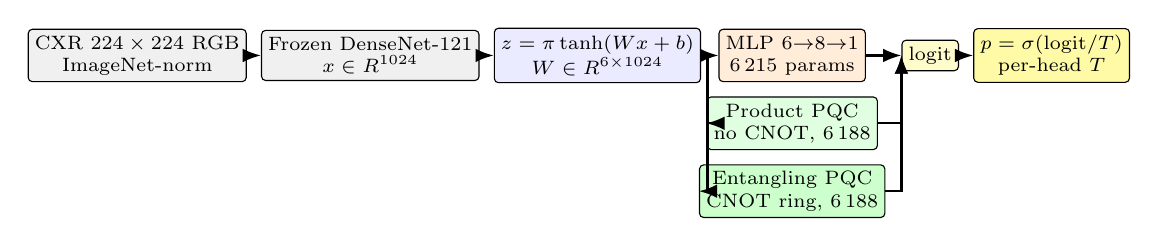
\begin{tikzpicture}[
      font=\scriptsize,
      box/.style={draw, rounded corners=1.5pt, align=center, inner sep=2.4pt},
      arr/.style={-{Latex}, thick}
    ]
    \node[box, fill=gray!12] (img) {CXR $224\times224$ RGB\\ImageNet-norm};
    \node[box, fill=gray!12, right=0.18cm of img] (dn) {Frozen DenseNet-121\\$x\in\mathbb{R}^{1024}$};
    \node[box, fill=blue!8, right=0.18cm of dn] (z) {$z=\pi\tanh(Wx+b)$\\$W\in\mathbb{R}^{6\times1024}$};
    \node[box, fill=orange!15, right=0.22cm of z] (mlp) {MLP $6{\to}8{\to}1$\\6\,215 params};
    \node[box, fill=green!12, below=0.18cm of mlp] (prod) {Product PQC\\no CNOT, 6\,188};
    \node[box, fill=green!20, below=0.18cm of prod] (ent) {Entangling PQC\\CNOT ring, 6\,188};
    \node[box, fill=yellow!20, right=0.45cm of mlp] (y) {logit};
    \node[box, fill=yellow!35, right=0.18cm of y] (t) {$p=\sigma(\mathrm{logit}/T)$\\per-head $T$};
    \draw[arr] (img) -- (dn);
    \draw[arr] (dn) -- (z);
    \draw[arr] (z) -- (mlp);
    \draw[arr] (z.east) -- ++(0.08,0) |- (prod.west);
    \draw[arr] (z.east) -- ++(0.08,0) |- (ent.west);
    \draw[arr] (mlp) -- (y);
    \draw[arr] (prod.east) -- (prod.east -| y.west) -- (y.west);
    \draw[arr] (ent.east) -- (ent.east -| y.west) -- (y.west);
    \draw[arr] (y) -- (t);
  \end{tikzpicture}}}
\end{figure}

\begin{figure}[ht]
\floatconts
  {fig:circuits}
  {\caption{PQC heads as implemented. Angle embedding is $\mathrm{RY}(z_i)$ on wires $q_0,\ldots,q_5$. Each of two layers applies RX/RY/RZ on every wire. The product head stops there. The entangling head then applies a sequential ring $\mathrm{CNOT}(0,1),\ldots,\mathrm{CNOT}(4,5),\mathrm{CNOT}(5,0)$---six two-qubit gates, not a multi-target CNOT. Readout is $\langle Z_0\rangle$, then a learned scale and bias.}}
  {\resizebox{0.98\linewidth}{!}{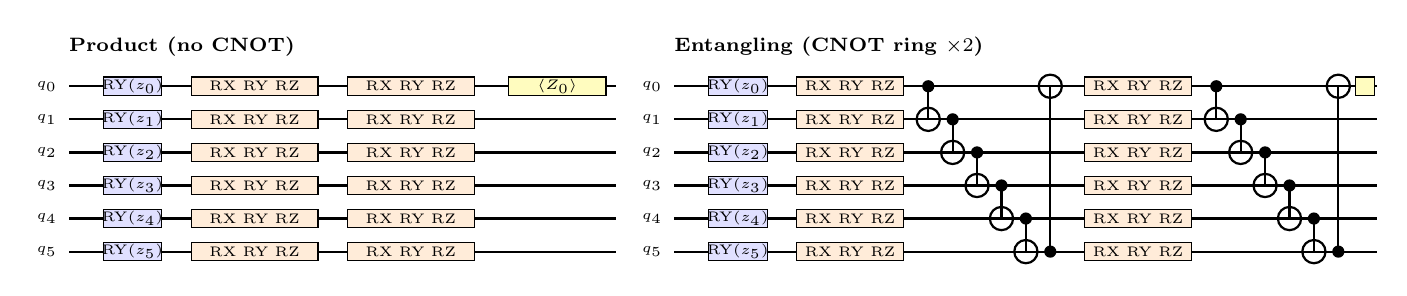
\begin{tikzpicture}[font=\tiny, x=0.62cm, y=0.42cm]
    % Product
    \node[anchor=west, font=\scriptsize\bfseries] at (-0.2,7.2) {Product (no CNOT)};
    \foreach \q in {0,1,2,3,4,5} {
      \draw[thick] (0,{6-\q}) -- (11.2,{6-\q});
      \node[anchor=east] at (-0.05,{6-\q}) {$q_{\q}$};
      \draw[fill=blue!12] (0.7,{6-\q-0.28}) rectangle (1.9,{6-\q+0.28});
      \node at (1.3,{6-\q}) {$\mathrm{RY}(z_{\q})$};
      \draw[fill=orange!15] (2.5,{6-\q-0.28}) rectangle (5.1,{6-\q+0.28});
      \node at (3.8,{6-\q}) {RX RY RZ};
      \draw[fill=orange!15] (5.7,{6-\q-0.28}) rectangle (8.3,{6-\q+0.28});
      \node at (7.0,{6-\q}) {RX RY RZ};
    }
    \draw[fill=yellow!25] (9.0,5.72) rectangle (11.0,6.28);
    \node at (10.0,6.0) {$\langle Z_0\rangle$};
    % Entangling
    \begin{scope}[shift={(12.4,0)}]
    \node[anchor=west, font=\scriptsize\bfseries] at (-0.2,7.2) {Entangling (CNOT ring $\times 2$)};
    \foreach \q in {0,1,2,3,4,5} {
      \draw[thick] (0,{6-\q}) -- (14.4,{6-\q});
      \node[anchor=east] at (-0.05,{6-\q}) {$q_{\q}$};
      \draw[fill=blue!12] (0.7,{6-\q-0.28}) rectangle (1.9,{6-\q+0.28});
      \node at (1.3,{6-\q}) {$\mathrm{RY}(z_{\q})$};
      \draw[fill=orange!15] (2.5,{6-\q-0.28}) rectangle (4.7,{6-\q+0.28});
      \node at (3.6,{6-\q}) {RX RY RZ};
    }
    % ring 1: sequential CNOTs as dots+targets
    \foreach \i/\j/\x in {0/1/5.2,1/2/5.7,2/3/6.2,3/4/6.7,4/5/7.2} {
      \fill (\x,{6-\i}) circle (2.2pt);
      \draw[thick] (\x,{6-\i}) -- (\x,{6-\j});
      \draw[thick] (\x,{6-\j}) circle (4.2pt);
    }
    \fill (7.7,1.0) circle (2.2pt);
    \draw[thick] (7.7,1.0) -- (7.7,6.0);
    \draw[thick] (7.7,6.0) circle (4.2pt);
    \foreach \q in {0,1,2,3,4,5} {
      \draw[fill=orange!15] (8.4,{6-\q-0.28}) rectangle (10.6,{6-\q+0.28});
      \node at (9.5,{6-\q}) {RX RY RZ};
    }
    \foreach \i/\j/\x in {0/1/11.1,1/2/11.6,2/3/12.1,3/4/12.6,4/5/13.1} {
      \fill (\x,{6-\i}) circle (2.2pt);
      \draw[thick] (\x,{6-\i}) -- (\x,{6-\j});
      \draw[thick] (\x,{6-\j}) circle (4.2pt);
    }
    \fill (13.6,1.0) circle (2.2pt);
    \draw[thick] (13.6,1.0) -- (13.6,6.0);
    \draw[thick] (13.6,6.0) circle (4.2pt);
    \draw[fill=yellow!25] (13.95,5.72) rectangle (14.35,6.28);
    \end{scope}
  \end{tikzpicture}}}
\end{figure}

\subsection{Training, calibration, and metrics}

Heads are trained with Adam \cite{kingma2015adam} ($\mathrm{lr}=10^{-3}$, weight decay $10^{-4}$), binary cross-entropy with logits, 40 epochs, and early stopping of 8 epochs on validation AUROC. MLP batches are size 64 on CUDA when available; PQC batches are size 16 on CPU. Seeds are 42, 43, and 44. The same CheXpert validation split is then reused to fit a scalar temperature $T=\exp(\theta)$ by L-BFGS on validation logits \cite{guo2017calibration}; CheXpert test and VinDr-CXR are never used for model selection or for $T$.
\begin{equation}
\label{eq:temperature}
\theta^{\star}=\arg\min_{\theta}\ \mathrm{BCE}\!\left(y,\ \sigma\!\left(z/\exp(\theta)\right)\right),\qquad T=\exp(\theta)\in[10^{-3},100].
\end{equation}
Calibrated probabilities use $\sigma(\mathrm{logit}/T)$. Metrics: AUROC, AUPRC, F1 at threshold 0.5, Brier score, and 15-bin ECE/MCE,
\begin{equation}
\label{eq:ece}
\mathrm{ECE}=\sum_{b=1}^{B}\frac{n_b}{n}\bigl|\mathrm{acc}(b)-\mathrm{conf}(b)\bigr|,
\end{equation}
with equal-width bins on $[0,1]$. JSON records do not store logits; reliability diagrams are recomputed from checkpoints. A run is $T$-degenerate if the optimizer hit the clamp. Those seven runs are retained in the main table and removed only in Appendix~\ref{app:degenerate}.

A fully trained DenseNet classifier is an unmatched upper bound. Fine-tuning the backbone, adding qubits mid-grid, merging pneumonia with consolidation in the main table, or describing PQC AUROC as quantum advantage would break the protocol.

\section{Experiments}

Forty-five of forty-five scheduled runs finished. VinDr metrics are present for every run. Mean $\pm$ standard deviation is over three seeds. Discrimination is in \tableref{tab:auroc}; calibration is in \tableref{tab:ece}; paired differences versus the matched MLP are in \tableref{tab:paired}. \figureref{fig:bars} shows the same means with seed error bars. The prose below states the pattern; the tables carry the numbers.

\subsection{Discrimination is comparable, not better}

On CheXpert test data the MLP is at least as discriminative as either PQC on every primary task (\tableref{tab:auroc}). The cleanest ontology is no finding: the three heads sit within a few points of one another, with the MLP slightly ahead. Under VinDr balanced evaluation the ranking is not reversed in a way that would support a quantum story. Product PQC is not uniformly worse on the target---consolidation is the one cell where it is numerically higher---but that gap sits inside seed noise. Across the 12 primary task--seed pairs, product AUROC is below the matched MLP on 9 CheXpert tests and entangling AUROC is below the MLP on 10. Mean paired $\Delta$AUROC versus MLP is negative for both heads on the source (\tableref{tab:paired}). Three seeds do not support a hierarchical significance test; the pattern is reported as paired mean differences, not as $p$-values.

\subsection{Entanglement is not a calibrator}

The primary question is calibration, not ranking AUROC. Entangling circuits do not yield lower source ECE (\tableref{tab:ece}; \figureref{fig:bars}). Where a PQC is better calibrated on CheXpert, it is the product circuit---no finding and pleural effusion---not the CNOT ring. The entangling head on no finding seed 42 is the clearest single-run illustration: it over-predicts the positive class (accuracy $0.560$, sensitivity $0.951$, ECE $0.419$; \figureref{fig:reliability}). Ring CNOTs at two layers and a single-qubit readout increase expressibility in the sense of Sim et al.\ \cite{sim2019expressibility}; they do not give the optimizer a calibration incentive. Across the 12 primary pairs, product ECE is lower than MLP ECE on 8 CheXpert tests; entangling ECE is lower on only 3. On VinDr balanced data, raw ECE is sometimes lower for PQC heads, but that reduction coexists with weaker or comparable AUROC and does not survive temperature transfer.

\subsection{Source-fitted temperature need not travel}

Temperature fitted on CheXpert validation is not a reliable target calibrator (\figureref{fig:transfer}). The intended use of Guo-style scaling is to correct overconfidence on a held-out slice of the same corpus. CheXpert validation and test are natural-prevalence slices of that US corpus; VinDr balanced evaluation forces prevalence $0.5$ (or $0.353$ for consolidation). A scalar $T$ cannot undo a prevalence and device shift \cite{ovadia2019shift,guo2017calibration}. On no finding product PQC, mean CheXpert ECE falls after scaling while VinDr balanced ECE rises---the same $T$ helps the source and harms the target. Seven of 45 runs hit the clamp $T\in\{0.001,100\}$ (\tableref{tab:degenerate}): cardiomegaly entangling seed 43 ($T=100$); consolidation MLP seed 43 ($T=100$); consolidation product seeds 42 ($T=0.001$) and 44 ($T=100$); and three pneumonia-proxy runs in the appendix. Those fits flatten or sharpen probabilities until ECE on one domain is a box-constraint artifact. They remain in \tableref{tab:ece}. Removing them does not reverse the no-finding or pleural-effusion rankings, where $n_{\mathrm{deg}}=0$. The cardiomegaly entangling VinDr-balanced calibrated ECE of $0.039\pm0.064$ is dominated by the $T=100$ run (calibrated ECE $\approx 0$) and is not evidence of successful transfer. Source-fitted $T$ does not systematically help PQC more than MLP on VinDr-CXR.

\texttt{pneumonia\_proxy} CheXpert test prevalence is $0.024$ (12 positives in 500). AUROC numbers on that split are high-variance and are not pneumonia performance (\tableref{tab:appendix}).

\begin{table}[ht]
\floatconts
  {tab:splits}
  {\caption{Frozen evaluation-split sizes. Train is class-balanced at $n=2000$. VinDr balanced consolidation is 353/647. Splits were not resampled after the grid.}}
  {\small\begin{tabular}{lrrrrrr}
  \toprule
  Task & CheX.\ $n_+$ & prev. & VinDr-bal $n_+$ & prev. & VinDr-nat $n_+$ & prev. \\
  \midrule
  No finding & 41 & 0.082 & 500 & 0.500 & 702 & 0.702 \\
  Cardiomegaly & 63 & 0.126 & 500 & 0.500 & 164 & 0.164 \\
  Pleural effusion & 225 & 0.450 & 500 & 0.500 & 62 & 0.062 \\
  Consolidation & 35 & 0.070 & 353 & 0.353 & 27 & 0.027 \\
  Pneumonia proxy & 12 & 0.024 & 500 & 0.500 & 55 & 0.055 \\
  \bottomrule
  \end{tabular}}
\end{table}

\begin{table}[ht]
\floatconts
  {tab:auroc}
  {\caption{Discrimination (secondary). Mean$\pm$std over seeds $\{42,43,44\}$. AUROC on raw logits.}}
  {\small\begin{tabular}{llccc}
  \toprule
  Task & Head & AUROC CheXpert & AUROC VinDr-bal & AUROC VinDr-nat \\
  \midrule
  No finding & MLP & $0.837\pm0.003$ & $0.736\pm0.008$ & $0.736\pm0.015$ \\
  No finding & Product & $0.820\pm0.007$ & $0.669\pm0.003$ & $0.667\pm0.012$ \\
  No finding & Entangling & $0.813\pm0.010$ & $0.725\pm0.015$ & $0.729\pm0.009$ \\
  Cardiomegaly & MLP & $0.681\pm0.005$ & $0.774\pm0.012$ & $0.757\pm0.014$ \\
  Cardiomegaly & Product & $0.637\pm0.036$ & $0.772\pm0.028$ & $0.768\pm0.019$ \\
  Cardiomegaly & Entangling & $0.679\pm0.006$ & $0.765\pm0.021$ & $0.756\pm0.022$ \\
  Pleural effusion & MLP & $0.761\pm0.004$ & $0.665\pm0.018$ & $0.659\pm0.004$ \\
  Pleural effusion & Product & $0.752\pm0.018$ & $0.643\pm0.010$ & $0.625\pm0.013$ \\
  Pleural effusion & Entangling & $0.748\pm0.011$ & $0.619\pm0.035$ & $0.614\pm0.011$ \\
  Consolidation & MLP & $0.652\pm0.030$ & $0.682\pm0.035$ & $0.680\pm0.048$ \\
  Consolidation & Product & $0.642\pm0.026$ & $0.714\pm0.012$ & $0.691\pm0.028$ \\
  Consolidation & Entangling & $0.613\pm0.033$ & $0.604\pm0.056$ & $0.586\pm0.073$ \\
  \bottomrule
  \end{tabular}}
\end{table}

\begin{table}[ht]
\floatconts
  {tab:ece}
  {\caption{Calibration (primary). 15-bin ECE, mean$\pm$std. $T$ is fitted on CheXpert validation only. $n_{\mathrm{deg}}$ counts runs with $T\in\{0.001,100\}$.}}
  {\small\setlength{\tabcolsep}{4pt}\begin{tabular}{@{}llccc@{}}
  \toprule
  Task & Head & ECE CheXpert & ECE VinDr-bal & $n_{\mathrm{deg}}$ \\
       & & raw$\to$cal & raw$\to$cal & \\
  \midrule
  No finding & MLP & $0.320\pm0.069\to0.317\pm0.105$ & $0.250\pm0.081\to0.207\pm0.038$ & 0 \\
  No finding & Product & $0.239\pm0.031\to0.153\pm0.087$ & $0.124\pm0.011\to0.203\pm0.049$ & 0 \\
  No finding & Entangling & $0.379\pm0.038\to0.375\pm0.050$ & $0.200\pm0.021\to0.151\pm0.077$ & 0 \\
  Cardiomegaly & MLP & $0.276\pm0.082\to0.219\pm0.134$ & $0.187\pm0.069\to0.263\pm0.131$ & 0 \\
  Cardiomegaly & Product & $0.315\pm0.076\to0.262\pm0.160$ & $0.105\pm0.091\to0.152\pm0.168$ & 0 \\
  Cardiomegaly & Entangling & $0.422\pm0.048\to0.376\pm0.001$ & $0.093\pm0.021\to0.039\pm0.064$ & 1 \\
  Pleural effusion & MLP & $0.112\pm0.036\to0.092\pm0.034$ & $0.160\pm0.076\to0.118\pm0.077$ & 0 \\
  Pleural effusion & Product & $0.072\pm0.005\to0.075\pm0.012$ & $0.178\pm0.014\to0.187\pm0.024$ & 0 \\
  Pleural effusion & Entangling & $0.105\pm0.032\to0.100\pm0.036$ & $0.105\pm0.051\to0.091\pm0.030$ & 0 \\
  Consolidation & MLP & $0.417\pm0.047\to0.386\pm0.047$ & $0.107\pm0.040\to0.115\pm0.034$ & 1 \\
  Consolidation & Product & $0.362\pm0.102\to0.300\pm0.196$ & $0.085\pm0.029\to0.200\pm0.134$ & 2 \\
  Consolidation & Entangling & $0.407\pm0.011\to0.408\pm0.021$ & $0.073\pm0.029\to0.096\pm0.029$ & 0 \\
  \bottomrule
  \end{tabular}}
\end{table}

\begin{table}[ht]
\floatconts
  {tab:paired}
  {\caption{Paired differences versus the matched MLP (12 primary pairs). Negative $\Delta$AUROC: PQC worse. Negative $\Delta$ECE: PQC better calibrated. No $p$-values ($n=3$ seeds).}}
  {\small\setlength{\tabcolsep}{3.5pt}\begin{tabular}{@{}lcccccc@{}}
  \toprule
  Head & $\Delta$AUROC & $\Delta$ECE & $\Delta$AUROC & $\Delta$ECE & worse & better \\
       & src & src & tgt & tgt & AUROC & ECE \\
  \midrule
  Product & $-0.020\pm0.034$ & $-0.034\pm0.084$ & $-0.015\pm0.042$ & $-0.053\pm0.082$ & 9/12 & 8/12 \\
  Entangling & $-0.019\pm0.030$ & $+0.047\pm0.087$ & $-0.036\pm0.048$ & $-0.058\pm0.077$ & 10/12 & 3/12 \\
  \bottomrule
  \end{tabular}}
\end{table}

\begin{figure}[ht]
\floatconts
  {fig:bars}
  {\caption{Grouped bars (mean over three seeds; error bars $=$ std) for MLP, product PQC, and entangling PQC. Pneumonia proxy is excluded.}}
  {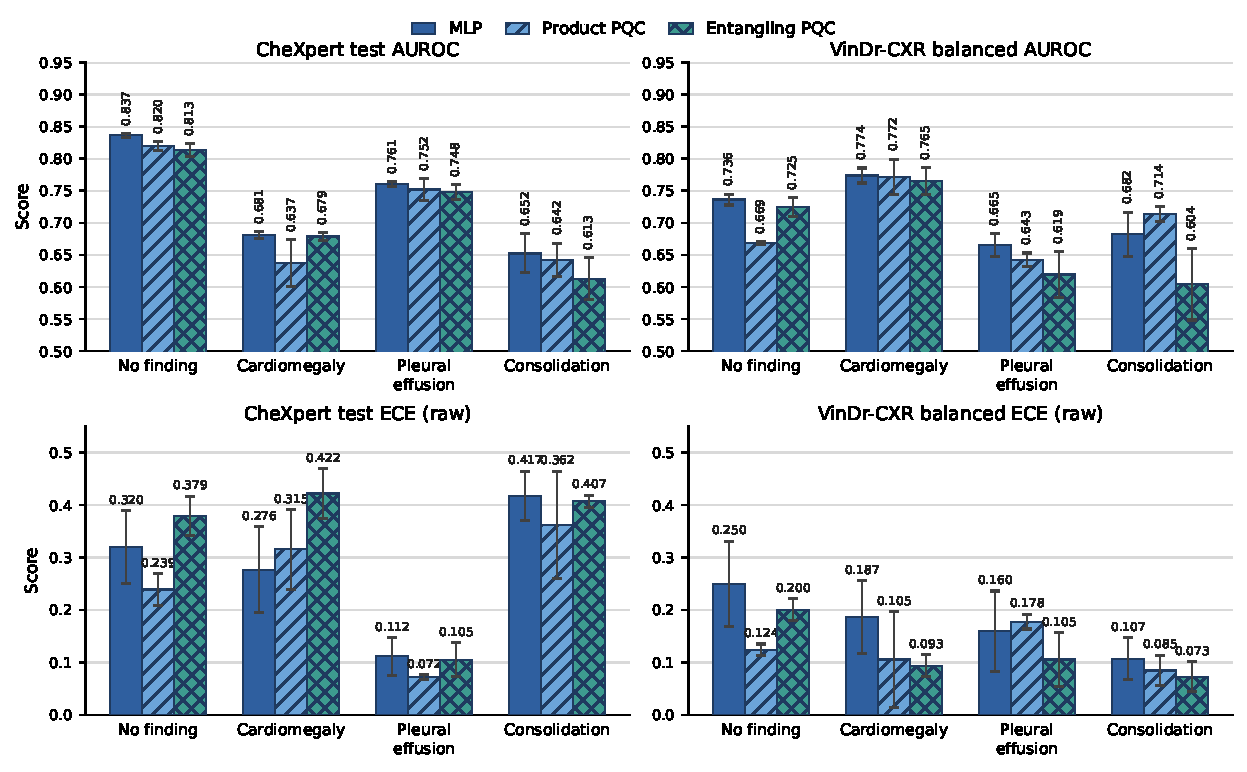
\includegraphics[width=0.98\linewidth]{figures/fig_auroc_ece_bars.pdf}}
\end{figure}

\begin{figure}[ht]
\floatconts
  {fig:transfer}
  {\caption{Change in ECE after source-fitted temperature scaling on the 36 primary runs. Lower-left: both domains improve. Upper-left: CheXpert improves and VinDr-CXR degrades.}}
  {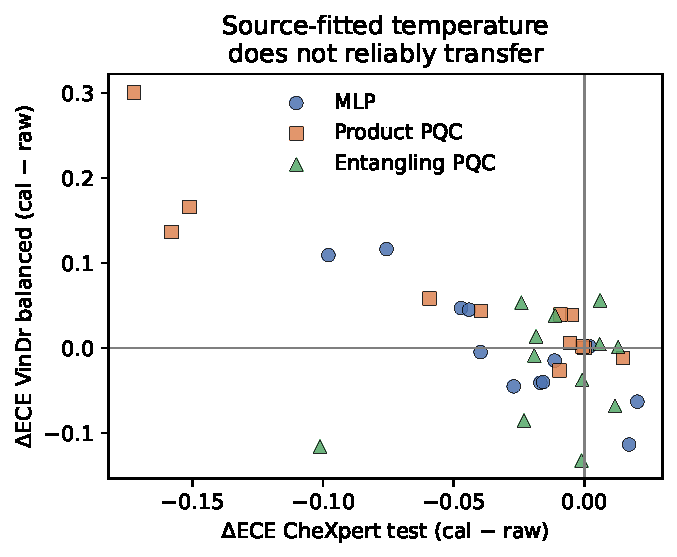
\includegraphics[width=0.52\linewidth]{figures/fig_temperature_transfer.pdf}}
\end{figure}

\begin{figure}[ht]
\floatconts
  {fig:reliability}
  {\caption{Reliability diagrams for no finding, seed 42. Marker area $\propto$ bin mass. Entangling PQC over-predicts the positive class on CheXpert test (accuracy $0.56$, ECE $0.419$).}}
  {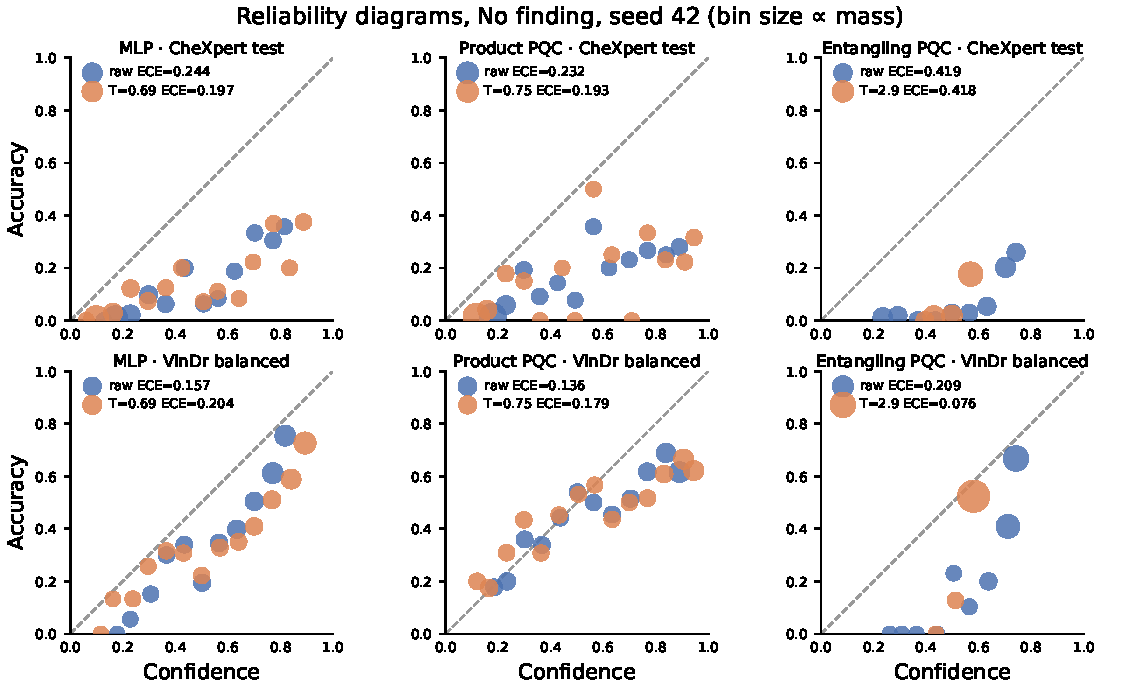
\includegraphics[width=0.92\linewidth]{figures/fig_reliability_no_finding_seed42.pdf}}
\end{figure}

\section{Discussion}

The protocol answers a smaller question than hybrid-imaging abstracts usually ask, and the answer is negative. A six-qubit expectation head is not a more trustworthy replacement for a 65-parameter MLP sitting on the same six angles. That is not a statement about quantum machine learning in general. It is a statement about this ansatz, this readout, this frozen trunk, this sample size, and this shift.

Two inductive-bias observations follow. First, the product circuit---not the entangling circuit---is the PQC that occasionally lowers source ECE (no finding, pleural effusion). Bounded $\langle Z_0\rangle\in[-1,1]$ plus a learned scale and bias is a different hypothesis class from an unconstrained MLP; it is not automatically better, and it is not entanglement. Second, adding a CNOT ring at two layers with a single-qubit observable increases expressibility without giving the optimizer a calibration incentive. On no finding seed 42 the entangling head becomes a high-sensitivity, low-accuracy over-predictor.

Temperature scaling fails for a structural reason that does not require a quantum story. A scalar $T$ fitted to source negative log-likelihood cannot undo a prevalence and device shift. When $T$ hits $0.001$ or $100$, ECE on one domain becomes a box-constraint artifact. Reporting those runs, rather than dropping them, is part of the result.

VinDr-CXR has no Pneumonia class. Mapping CheXpert Pneumonia onto Consolidation $\cup$ Infiltration changes the label definition. We leave that task in the appendix with the flag the code already carries.

\section{Limitations}

The circuit has six qubits, two layers, and a single observable. The backbone is frozen, so the PQC never sees pixels. Simulation uses \texttt{default.qubit}, not hardware noise. Sample sizes are small (train 2\,000; val/test 500; VinDr 1\,000). Three seeds cannot support a confirmatory hypothesis test. Temperature is a scalar with a hard clamp. ECE uses 15 equal-width bins; rare positives make several bins empty \cite{nixon2019measuring}. VinDr any-vote ignores radiologist disagreement. ImageNet-normalized $224\times 224$ RGB conversion is a crude CXR preprocessing. No clinical deployment is claimed.

\section{Conclusion}

Under the protocol actually run---frozen ImageNet DenseNet-121, shared $z\in\mathbb{R}^{6}$, six-qubit two-layer product and ring-CNOT heads, noiseless \texttt{default.qubit}, three seeds---neither PQC head is a more trustworthy replacement for the matched MLP on CheXpert $\to$ VinDr-CXR. Discrimination is comparable or slightly worse. Entanglement does not reduce ECE. Source-fitted temperature scaling can harm the target. Those are empirical boundaries for this capacity and shift, not evidence against quantum machine learning in general.

\clearpage
\midlacknowledgments{No external funding was received. The author thanks the maintainers of CheXpert and VinDr-CXR for releasing de-identified public datasets. Large language models were used only for copy-editing; the author is responsible for all scientific content, numbers, and claims.}

\bibliographystyle{plainnat}
\bibliography{references}

\appendix

\section{Pneumonia proxy (ontology shift)}

\begin{table}[h]
\floatconts
  {tab:appendix}
  {\caption{\texttt{pneumonia\_proxy} maps CheXpert Pneumonia to VinDr Consolidation $\cup$ Infiltration. Not a pneumonia detector. Product ECE collapse on CheXpert coexists with two $T=0.001$ seeds.}}
  {\setlength{\tabcolsep}{4pt}\begin{tabular}{@{}lcccc@{}}
  \toprule
  Head & AUROC CheX. & ECE CheX. & AUROC VinDr-bal & ECE VinDr \\
       & & raw$\to$cal & & raw$\to$cal \\
  \midrule
  MLP & $0.662\pm0.071$ & $0.467\to0.436$ & $0.629\pm0.044$ & $0.059\to0.024$ \\
  Product & $0.625\pm0.072$ & $0.338\to0.099$ & $0.582\pm0.062$ & $0.113\to0.446$ \\
  Entangling & $0.711\pm0.032$ & $0.438\to0.437$ & $0.609\pm0.025$ & $0.087\to0.083$ \\
  \bottomrule
  \end{tabular}}
\end{table}

\section{$T$-degenerate runs}
\label{app:degenerate}

\begin{table}[h]
\floatconts
  {tab:degenerate}
  {\caption{Runs whose L-BFGS temperature hit the clamp. Retained in the main tables. Cardiomegaly entangling seed 43 VinDr-balanced calibrated ECE $\approx 0$ is a $T=100$ artifact.}}
  {\setlength{\tabcolsep}{4pt}\begin{tabular}{@{}llrcc@{}}
  \toprule
  Task & Head & Seed & $T$ & ECE CheX.\ / VinDr-bal \\
       & & & & raw/cal \\
  \midrule
  Cardiomegaly & Entangling & 43 & 100 & 0.476/0.375 \quad 0.116/0.000 \\
  Consolidation & MLP & 43 & 100 & 0.470/0.430 \quad 0.152/0.147 \\
  Consolidation & Product & 42 & 0.001 & 0.246/0.074 \quad 0.051/0.352 \\
  Consolidation & Product & 44 & 100 & 0.439/0.430 \quad 0.107/0.147 \\
  Pneumonia proxy & MLP & 43 & 100 & 0.522/0.476 \quad 0.115/0.001 \\
  Pneumonia proxy & Product & 42 & 0.001 & 0.350/0.096 \quad 0.058/0.414 \\
  Pneumonia proxy & Product & 43 & 0.001 & 0.384/0.194 \quad 0.085/0.457 \\
  \bottomrule
  \end{tabular}}
\end{table}

Dropping these seven runs does not reverse the primary conclusions on no finding or pleural effusion ($n_{\mathrm{deg}}=0$). Consolidation product then has a single remaining seed; that cell is too thin to interpret.

\section{Additional reliability diagrams}

Reliability diagrams below are generated from dumped checkpoint logits, not from JSON.

\begin{figure}[h]
\floatconts
  {fig:rel-cardio}
  {\caption{Reliability diagrams, cardiomegaly, seed 42.}}
  {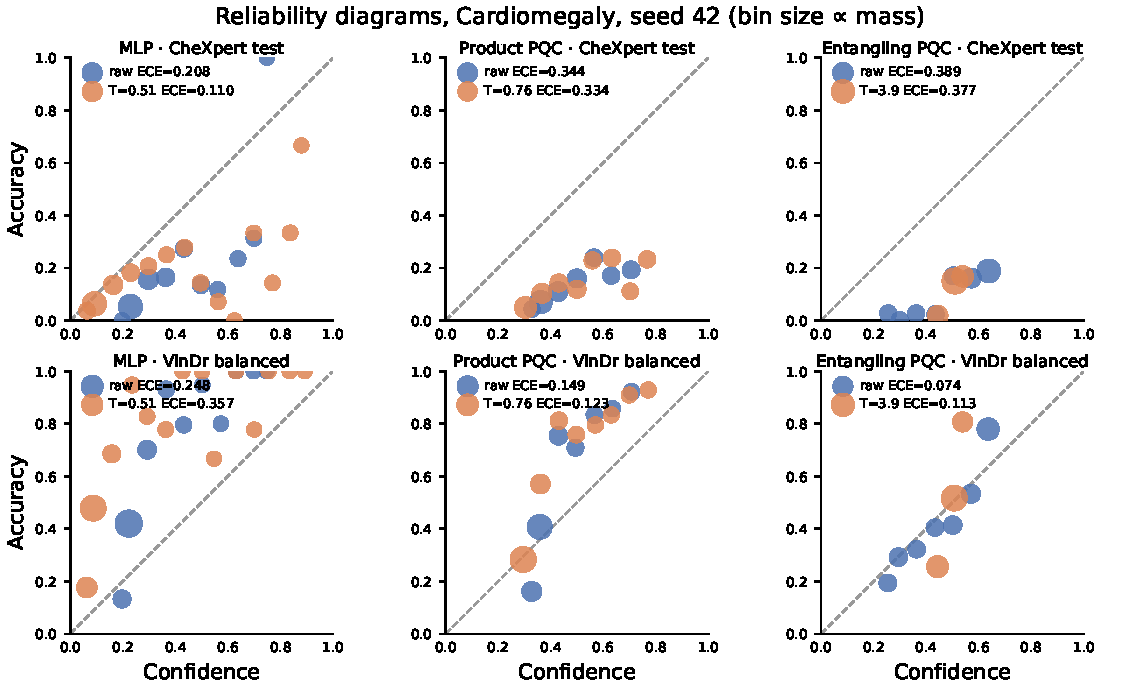
\includegraphics[width=0.88\linewidth]{figures/fig_reliability_cardiomegaly_seed42.pdf}}
\end{figure}

\begin{figure}[h]
\floatconts
  {fig:rel-pleural}
  {\caption{Reliability diagrams, pleural effusion, seed 42.}}
  {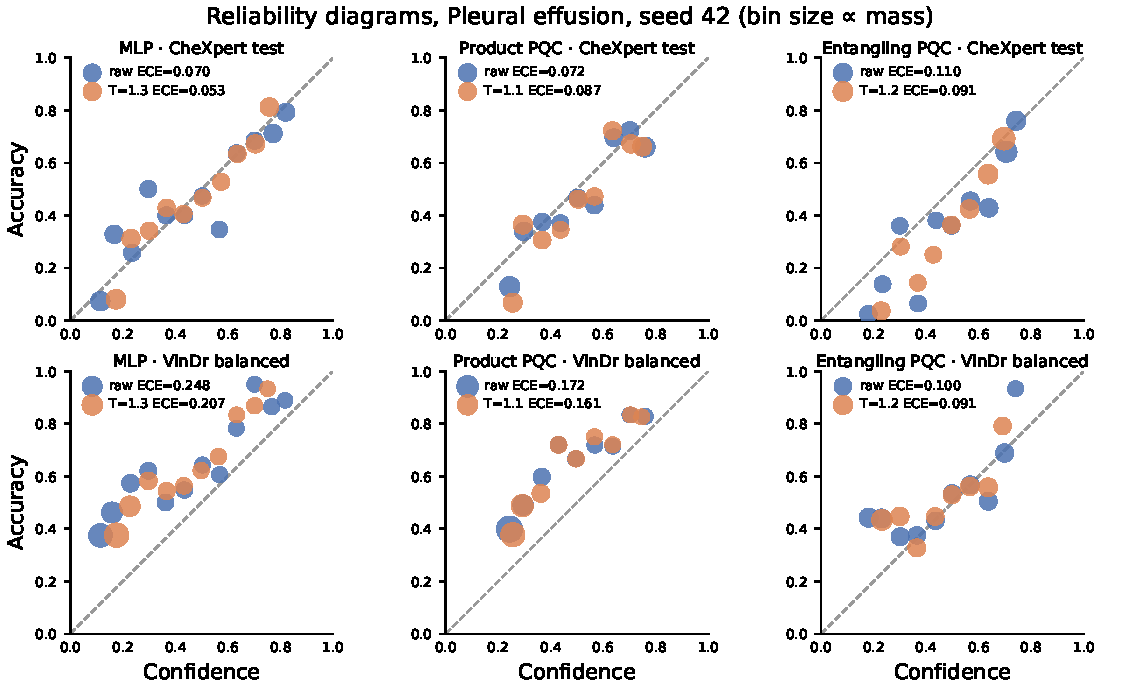
\includegraphics[width=0.88\linewidth]{figures/fig_reliability_pleural_effusion_seed42.pdf}}
\end{figure}

\begin{figure}[h]
\floatconts
  {fig:rel-cons}
  {\caption{Reliability diagrams, consolidation, seed 42.}}
  {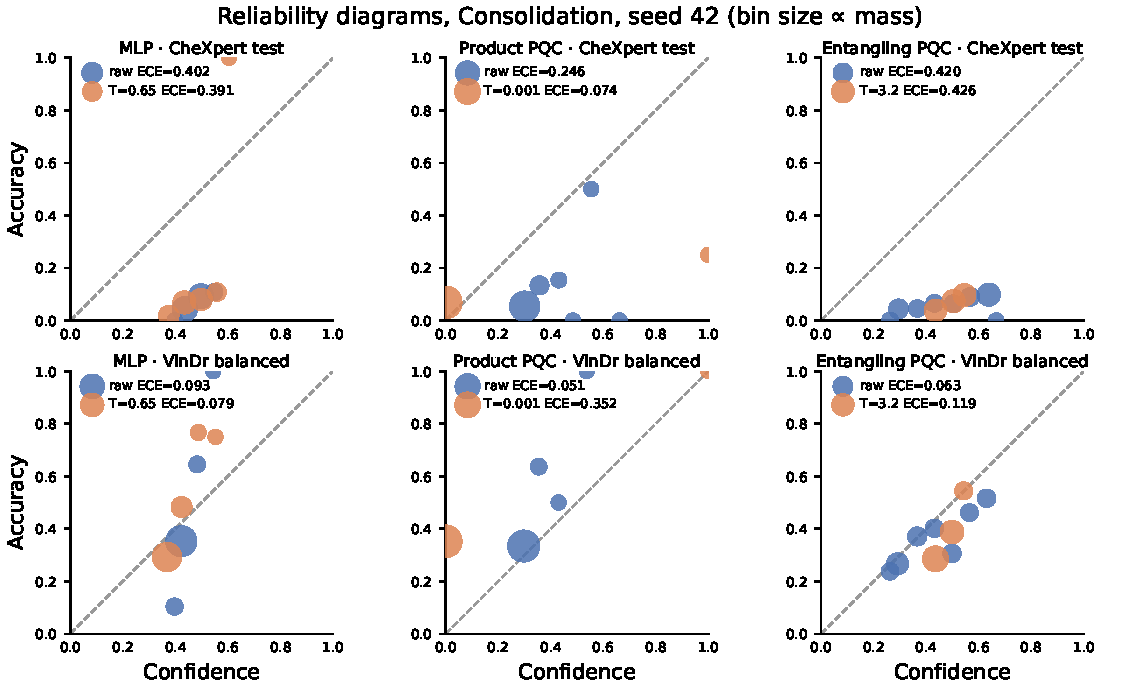
\includegraphics[width=0.88\linewidth]{figures/fig_reliability_consolidation_seed42.pdf}}
\end{figure}

\begin{figure}[h]
\floatconts
  {fig:rel-pna}
  {\caption{Reliability diagrams, pneumonia proxy, seed 42 (appendix task).}}
  {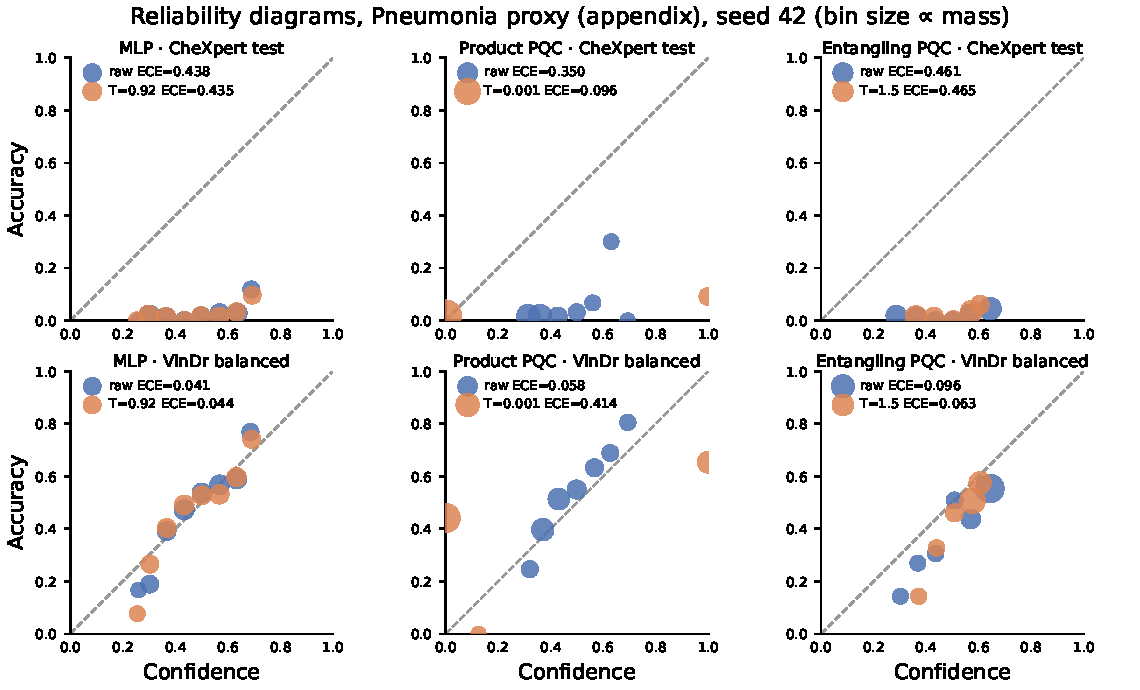
\includegraphics[width=0.88\linewidth]{figures/fig_reliability_pneumonia_proxy_seed42.pdf}}
\end{figure}

\section{Reproducibility}

Interpreter: Python 3.10, PyTorch 2.6.0+cu124, PennyLane 0.38.0. Config: \texttt{configs/default.yaml}. Grid: \texttt{scripts/run\_queue.py} (45/45 complete). Tables: \texttt{results/tables/all\_runs.csv}. Checkpoints: \texttt{results/runs/}. Splits were not resampled after the grid. Logits for reliability diagrams are dumped from checkpoints by \texttt{scripts/dump\_logits.py}. Training code, frozen split files, and run JSON will be released with the camera-ready version if the paper is accepted; they are not on a public repository at submission. CheXpert and VinDr-CXR are public de-identified datasets. The author has no competing interests.

\end{document}
